\chapter{PRIME Data Headend Server}
\section{Introducción}
PRIME Data Headend Server, en adelante <<PRIME DHE>>, es un producto software capaz de sustituir un concentrador de datos tradicional en una red PRIME. <<PRIME DHE>> implementa uno o varios concentradores virtuales en un equipo servidor completamente deslocalizado de la red que administra. En conjunción con el router <<Regesta PLC 3G>> (de la compañía <<Teldat>>) como nodo base de la red, el tandem creado está habilitado para operar completamente una red PRIME. Así, se hace innecesario la instalación física de concentradores de datos, ahorrando una parte importante en costes de mantenimiento e instalación.

Para entender como trabaja <<PRIME DHE>>  primero hay que conocer la estructura de una red <<PRIME>>. La figura \ref{fig:EstructuraPRIME} representa una topología típica de una red PRIME. Los elementos que actúan en ella son los siguientes:
\begin{description}
	\item[STG] El Sistema de Telegestión es el punto de entrada del usuario operador de la red. Este se encarga de pedir periódicamente a los concentradores los informes con las medidas de consumo, y solicitar la ejecución de órdenes. Todo ello a través de servicios web.
	\item[Router] El router es el enlace de comunicaciones entre el concentrador y el STG.
	\item[Concentrador] El concentrador por su parte está constantemente preguntando a los contadores sus medidas y ejecuta las órdenes e informes que le solicite el STG. Para ello, típicamente, disponen de dos interfaces de red: una para recibir y enviar al STG (a través del router); y otra para la comunicación PLC con los contadores (a través del nodo base).
	\item[Nodo Base] El nodo base es el enlace de comunicaciones entre los contadores y el concentrador a través de la línea eléctrica.
	\item[Contadores] Los contadores son el fin último de las <<Smart Grids>>, llevan la cuenta de la energía consumida y vertida en la red eléctrica, controlan la potencia máxima de salida hacia el consumidor, etc...
\end{description}

\begin{figure}[htbp]
	\centering
	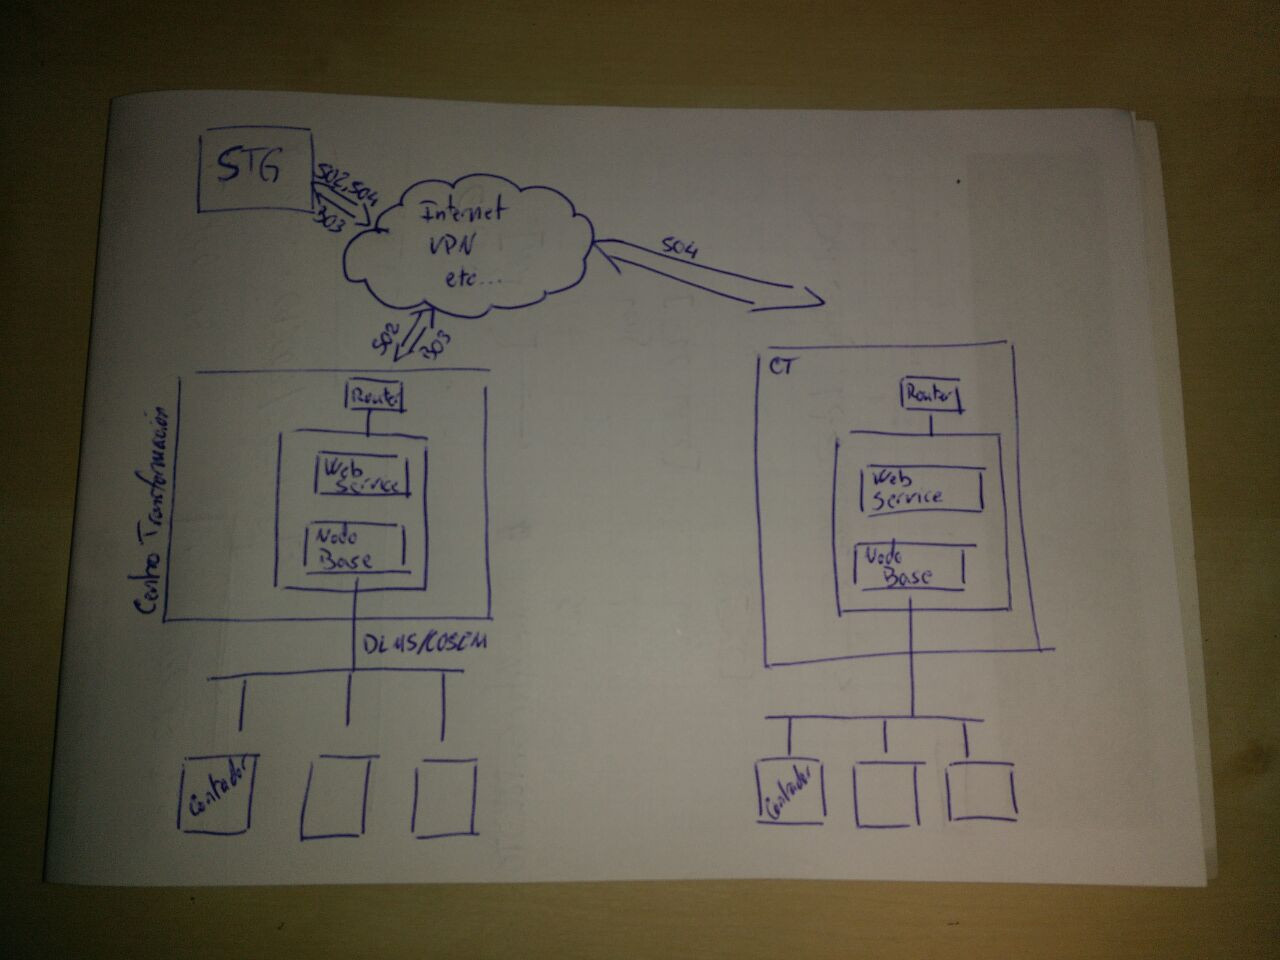
\includegraphics[width=\textwidth]{Img/boceto_estructura_prime.jpg}
	\caption{Topología de red PRIME}
	\label{fig:EstructuraPRIME}
\end{figure}

A grandes rasgos su funcionamiento sería el siguiente: el STG se comunica con el concentrador para solicitarle informes de medidas o la ejecución de alguna orden a través de los <<Web Services>>. El concentrador acepta las órdenes del STG, y las ejecuta comunicándose a su vez con los contadores a través del <<nodo base>> y enviando de nuevo la respuesta al STG. El concentrador también puede enviar informes de forma automática antes incluso de que el STG se los requiera.

En cualquier caso son bastantes dispositivos complejos los que entran en funcionamiento, con los costes de mantenimiento e instalación que conllevan. En este punto es dónde la propuesta de red de <<PRIME DHE>> muestra su primera ventaja. En la figura \ref{fig:EstructuraPrimeDHE} se observa la topología de red propuesta. En <<PRIME DHE>> se elimina el concentrador tradicional, y en su lugar se instala un router un tanto especial, este router contiene un nodo base PRIME al que podemos acceder para las comunicaciones con los contadores. Así, toda la lógica del concentrador es sustituida por <<PRIME DHE>>. Al ser un producto software, se pueden controlar varios nodos base con una sola instancia de <<PRIME DHE>>, con lo que se reducen los costes de operación, se homogeneiniza el funcionamiento y se gana en fiabilidad.

\begin{figure}[htbp]
	\centering
	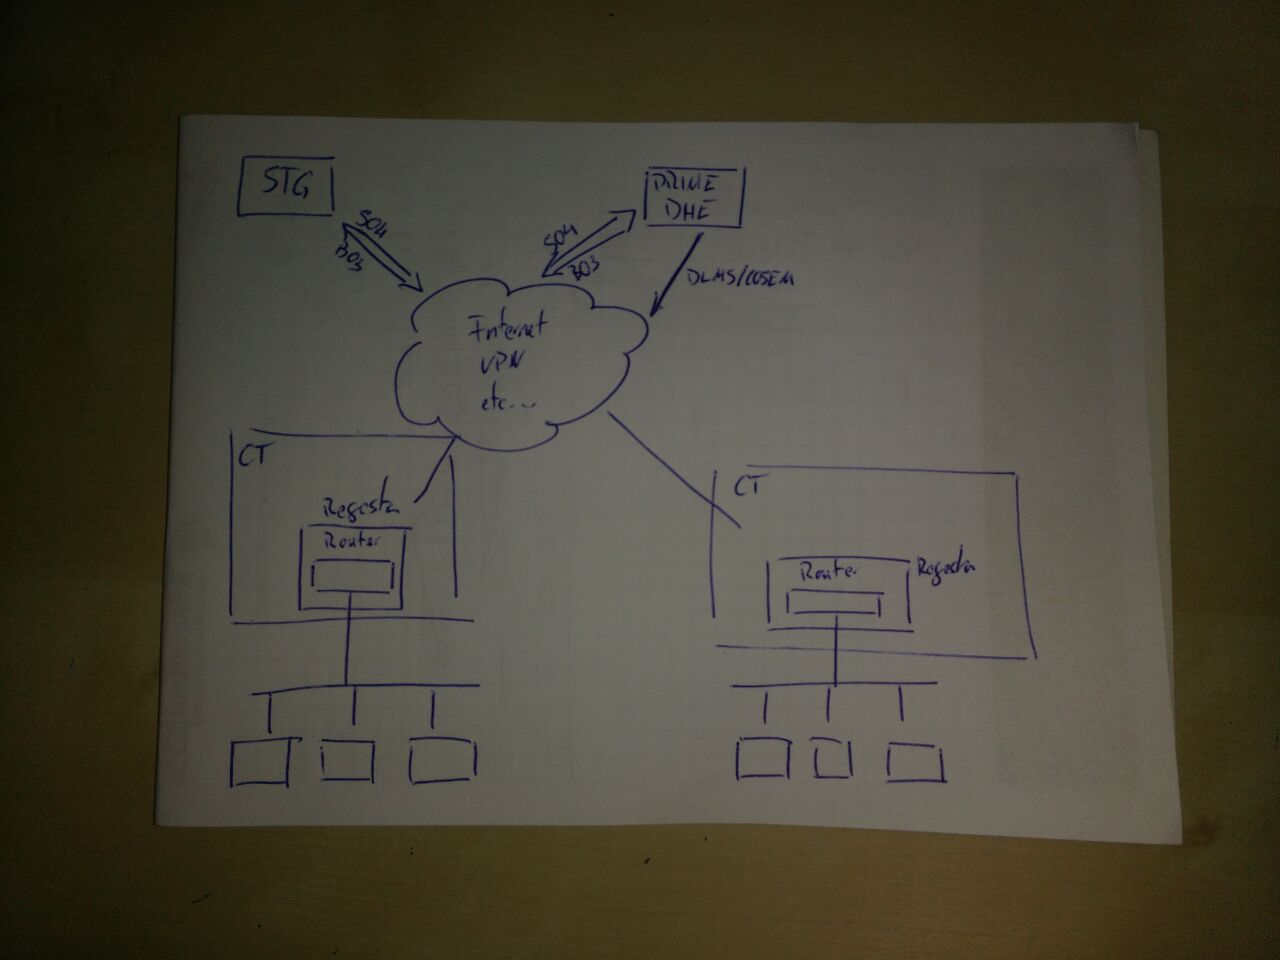
\includegraphics[width=\textwidth]{Img/boceto_red_primedhe.jpg}
	\caption{Topología de red PRIME DHE}
	\label{fig:EstructuraPrimeDHE}
\end{figure}

Por ello, la operativa tradicional bien se puede realizar por medio de un STG o bien por medio de la interfaz de la aplicación <<PRIME DHE>>. Según la topología mostrada, el sistema es perfectamente capaz de trabajar tanto con uno o con otro, o incluso pudiendo coexistir los dos a la vez. Esto propicia una adaptabilidad perfecta ante cualquier circunstancia o escenario posible.

La idea principal es la de abstraer toda complejidad posible, abarantando elementos físicos y, por ende, costes; sin que ello conlleve una disminución de características.

 Además, tal y como se puede ver en la imagen, <<PRIME DHE>> permite trabajar con más de un centro de transformación, permitiendo una modularidad e independencia de operaciones que antes no se conseguía. 
 
 \section{Arquitectura}
 
 <<PRIME DHE>> está diseñado siguiendo una arquitectura <<Cliente-Servidor>> multicapa. En líneas generales consiste en un software, al que llamaremos cliente, que realiza peticiones de datos u operaciones a otro software, al que llamaremos servidor. El servidor a su vez puede actuar como cliente de otro software servidor, etc.; repitiéndose el esquema por cada capa que compone el sistema. 
 
En este marco de funcionamiento la capacidad de proceso se reparte entre las distintas capas de clientes-servidores, con lo que se centraliza la gestión de la información y se fomenta la separación de responsabilidades; lo que facilita y clarifica el diseño del sistema.
 
 En resumen, esta arquitectura es la que mejor se adapta al escenario en el que nos movemos, ya que nos proporciona las siguientes ventajas:
 \begin{itemize}
 	\item Centralización del control
 	\item Alta escalabilidad
 	\item Fácil mantenimiento y ampliación
 	\item Mayor robustez y tolerancia a fallos
 	\item Mayor flexibilidad
 \end{itemize}

\subsection{Visión global}
Como hemos visto anteriormente, <<PRIME DHE>> esta estructurado en múltiples capas. En concreto son tres capas: la capa de usuario, la capa de gestión y procesamiento, y por último la capa de comunicaciones <<PRIME>>. En la figura \ref{fig:ArquitecturaDHEVisionGlobal} se puede ver una visión global del sistema.

\begin{figure}[htbp]
	\centering
	
\includegraphics[width=\textwidth]{Img/dummy.png}
	\caption{Arquitectura globlal <<PRIME DHE>>}
	\label{fig:ArquitecturaDHEVisionGlobal}
\end{figure}

\begin{description}
	\item[Capa usuario - <<VDC\_PRIME>>, aplicación web] La capa de usuario es el punto de entrada al sistema, tanto para usuarios humanos como para los <<STG>>, desde aquí se gestiona toda la interacción de los usuarios. La componen dos servicios: una aplicación web, que emula la interfaz de un concentrador tradicional, y <<VDC\_PRIME>> hace de interfaz para los STG. 
	\item[Capa de gestión y procesamiento - <<Thunder>>] Esta capa es el núcleo del sistema. Todas las peticiones se gestionan y procesan aquí. De ello se encarga <<Thunder>>, un gestor de tareas eficiente y versátil.
	\item[Capa de comunicaciones <<PRIME>> - <<Agamenón>>] En esta capa está contenida toda la lógica necesaria para las comunicaciones con los contadores. Esta capa está gobernada por <<Agamenón>>, un servicio que se encarga de traducir las peticiones en alto nivel a <<DLMS/COSEM>> que es el protocolo final en el que se intercambian los mensajes.
\end{description}

Cada capa tiene su propia base de datos, con lo que, la independencia y deslocalización de cada una de ellas está asegurada. De esta forma, podríamos tener un una máquina ejecutando los cuatro servicios y en otra las bases de datos. Otra opción podría se mantener las bases de datos en la nube y los servicios en un servidor más cerca de los dispositivos, o también una máquina para cada servicio. En cualquier caso, la flexibilidad del sistema en cuanto a requerimientos de despliegue y/o necesidades está asegurada.


\section{Agamenón}
Este servicio implementa la capa más baja del sistema. Su cometido, como vimos anteriormente, es encapsular la lógica de las comunicaciones <<PRIME>>. Así, ofrece el nivel de abstracción necesario para poder olvidarnos de los detalles específicos de esta tecnología como los reintentos, los códigos <<OBIS>>, etc...
\subsection{Comunicaciones}
<<Agamenón>> usa su base de datos como interfaz hacia el nivel superior. Cada registro nuevo en su base de datos lo trata como una petición independiente. Una vez insertada la petición, solo queda esperar a que acabe de procesarla y los datos requeridos ya estarán listos para su uso. La razón de este método de comunicación no es otra que la sencillez y la velocidad. 

En la operativa habitual (tanto para generar un informe como leer medidas de consumo) son necesarias bastantes peticiones distintas. La casuística de estas es muy amplia ya que pueden ser muchas distintas: para un solo contador, o la misma para muchos contadores, llegan a distintas velocidades, pueden no llegar siquiera, etc... Por todo ello, hay que hacer un seguimiento activo de cada una de las peticiones. Este seguimiento se podría volver muy engorroso si se dependiera de algún tipo de <<API>> o similar, en cambio, al ser las peticiones una tupla de una tabla en una base de datos, todos los actores implicados pueden interactuar con ella sin que se perjudique ni el rendimiento o la complejidad, y además evita colisiones.

\begin{table}[htbp]
	\centering
	\begin{tabular}{lll}
		\toprule
		Campo & Tipo de Dato & Uso\\ \toprule
		Id & Entero & Clave primaria \\ \cline{3-3}
		BaseNodeMAC & Cadena & \multirow{5}{*}{Datos <<PRIME>>} \\ 
		BaseNodeIP & Cadena & \\
		BaseNodePort & Cadena & \\
		ServiceNodeMAC & Cadena & \\
		ServiceNodePassword & Cadena & \\
		Data & Cadena & \\ \cline{3-3}
		Finish & Booleano & \multirow{9}{*}{Gestión de peticiones}\\
		FinishDateTime & Fecha y hora & \\
		FinishState & Entero & \\
		Retry & Entero & \\
		RetryInterval & Entero & \\
		NextRetryDate & Fecha y hora & \\
		Priority & Entero & \\
		TimeOutDateTime & Fecha y hora & \\
		Type & Entero & \\ \cline{3-3}
		Tracker & Entero & Seguimiento\\
		\bottomrule
	\end{tabular}
	\caption{Tabla para peticiones de Agamenón}
	\label{tab:DiagramaTablaAgamenon}
\end{table}

En la tabla \ref{tab:DiagramaTablaAgamenon} podemos ver resumidamente los campos que componen la tabla para las peticiones hacia <<Agamenón>> y su uso. Los nombres de los campos son bastante explícitos, no obstante, a continuación detallaremos los más relevantes.

\begin{description}
	\item[Datos <<PRIME>>] Estos se usan para identificar el dispositivo concreto del que se necesitan datos. IP y puerto de comunicaciones del Regesta asociado al <<nodo base>> y la MAC del contador para identificarlo dentro de la subred <<PRIME>>. <<Data>> es un objeto serializado que especifica el código <<Obis>> concreto a leer o escribir.
	\item[Gestión de peticiones] Con estos manejamos la petición. <<Finish>> indica si se ha terminado con la petición, <<FinishState>> muestra el estado de finalización, si ha sido exitosa o ha fallado; <<Retry>> indica el número de veces que se reintentará traer los datos y <<RetryInterval>> el tiempo mínimo entre reintentos. <<Priority>> se usa para establecer el orden en el que se ejecutarán las peticiones.
	\item[Seguimiento] <<Agamenón>> no usa el campo <<Tracker>>, este lo establece el peticionario de los datos para poder hacer el seguimiento de la o las peticiones.
\end{description}


\subsection{Estructura}
<<Agamenón>> está concebido para ser modular y estar desacoplado en cada una de sus partes. Lo cual, nos permite ampliarlo o modificarlo con un coste muy bajo. Principalmente, consta de cuatro piezas fundamentales que interactúan entre si: Engine, BaseNode, ServiceNode y ObisLibrary. En la figura \ref{fig:EstructuraAgameon} se puede ver un diagrama de la estructura general.
\begin{figure}[htbp]
	\centering
	
\includegraphics[width=\textwidth]{Img/dummy.png}
	\caption{Estructura <<Agamenón>>}
	\label{fig:EstructuraAgameon}
\end{figure}



\subsubsection{Engine}

El curso que sigue una petición comienza en el <<Engine>>. Este proceso es único y se está ejecutando ininterrumpidamente. Básicamente su función es seleccionar de la base de datos la siguiente petición a procesar e iniciar dicho proceso. Para ello busca las que cumplan con ciertos criterios: no estén terminadas, les queden reintentos, y le toque volver a intentarlo.

Una vez seleccionadas las candidatas se agrupan por <<Nodo Base>>, y se ordenan, primero por prioridad y luego por hora de siguiente reintento. Una vez hechas las listas, se seleccionan tantas peticiones como huecos libres tengan los <<Nodos Base>>. Para las seleccionadas, se les actualiza en base de datos el número de reintentos y la hora del próximo intento.

Para el siguiente paso del <<Engine>> hay dos opciones: levantar el <<Nodo Base>> y añadirle las peticiones, o bien, solo añadirle las peticiones. En cualquier caso, el trabajo del <<Engine>> acaba aquí, la responsabilidad del siguiente paso del proceso queda en manos del <<Nodo Base>>.

Un caso especial son las peticiones con <<proridad>> 1. Estas siempre son seleccionadas puesto que representan peticiones de muy alta proridad. Por ejemplo, los datos necesarios para crear un informe "S01". El cual se pide de forma síncrona, es decir, se espera que los datos vengan en la propia respuesta del servicio web, por lo que se necesita una respuesta del sistema casi inmediata.

\subsubsection{Ticket-67}\label{sec:ticket67}

Antes de seguir es necesario conocer un poco sobre <<Ticket-67>>.

En nuestro escenario, no tenemos acceso físico al nodo base que gobierna la red <<PRIME>>. En su lugar, nos comunicamos con el <<Regesta>> utilizando el protocolo <<Ticket-67>> sobre <<TCP/IP>>. En líneas generales este protocolo simplemente añade una cabecera para poder direccionar los mensajes <<DLMS>> e implementa unos cuantos comandos, o mensajes especiales a los que responde el propio nodo base, para una gestión básica de la red.

La cabecera de un mensaje en <<Ticket-67>> tiene el siguiente aspecto:

\begin{table}[h]
	\centering
	\begin{tabular}{cccccccc}
		\toprule
		0001 & 0001 & 0006 & 0005 & \multicolumn{4}{c}{001122334455}\\ \midrule
		Version & Source & Dest & Lenght & \multicolumn{4}{c}{DLMS} \\ 
		2 bytes & 2 bytes & 2 bytes & 2 bytes & \multicolumn{4}{c}{N bytes}\\
		\bottomrule
	\end{tabular}
	\caption{Cabecera <<Ticket-67>>}
	\label{tab:CabeceraTicket67}
\end{table}

\begin{description}
	\item[Version] Campo fijo que indica la versión de <<Ticket-67>> usada.
	\item[Source] Origen del mensaje. En el sentido <<PRIME DHE>> - <<Regesta>> es la dirección reservada \textsl{0001}(Client Management Process). En cambio, si es en el sentido <<Regesta>> - <<PRIME DHE>>, será la dirección del contador o \textsl{0000} si es el nodo base.
	\item[Dest] Destino del mensaje.
	\item[Lenght] Longitud del mensaje en bytes.
	\item[DLMS] El contenido del mensaje \textsl{DLMS}.
\end{description}

Entre los comandos disponibles cabe destacar:

Sentido <<PRIME DHE>> - <<Regesta>>
\begin{description}
	\item[START\_REPORTING\_METERS] Devuelve una lista con los contadores conectados actualmente, y habilita las notificaciones de conexión y desconexión de los contadores.
		\begin{table}[h]
			\centering
			\begin{tabular}{cccccccc}
				\midrule
				0001 & 0001 & 0000 & 0001 & \multicolumn{4}{c}{03}\\ \midrule
				Version & Source & Dest & Lenght & \multicolumn{4}{c}{Comando 03} \\ 
				\bottomrule
			\end{tabular}
		\end{table}
	\item[DELETE\_METERS] Fuerza la desconexión de un contador de la red.
	\begin{table}[h]
		\centering
		\begin{tabular}{cccccccc}
			\midrule
			0001 & 0001 & 0000 & 0003 & \multicolumn{4}{c}{040002}\\ \midrule
			Version & Source & Dest & Lenght & \multicolumn{4}{c}{Comando 04, identificador del contador 0002} \\ 
			\bottomrule
		\end{tabular}
	\end{table}
\end{description}


Sentido <<Regesta>> - <<PRIME DHE>>
\begin{description}
	\item[NEW\_DEVICE\_NOTIFICATION] Notifica un dispositivo nuevo en la red junto con su identificación(Identificador en la red, MAC, etc). 
	\begin{table}[h]
		\centering
		\begin{tabular}{cccccccc}
			\midrule
			0001 & 0000 & 0001 & 0019 & \multicolumn{4}{c}{010002...}\\ \midrule
			Version & Source & Dest & Lenght & \multicolumn{4}{c}{Comando 01, identificador del dispositivo 0002, ...} \\ 
			\bottomrule
		\end{tabular}
	\end{table}
	\item[REMOVE\_DEVICE\_NOTIFICATION] Notifica la desconexión de un contador de la red.
	\begin{table}[h]
		\centering
		\begin{tabular}{cccccccc}
			\midrule
			0001 & 0001 & 0000 & 0003 & \multicolumn{4}{c}{020002}\\ \midrule
			Version & Source & Dest & Lenght & \multicolumn{4}{c}{Comando 02, identificador del contador 0002} \\ 
			\bottomrule
		\end{tabular}
	\end{table}
\end{description}

El protocolo no es excesivamente complejo, pero requiere de cierto procesamiento a la hora de enviar y recibir mensajes, sobretodo, para abrir las comunicaciones y mantener el estado mientras duren. Así, el flujo de trabajo se podría definir en dos fases: inicialización y mantenimiento. 

En la fase inicialización, justo despues de abrir la conexión <<TCP/IP>>, hay que enviar el comando \textsl{START\_REPORTING\_METERS} para obtener la lista de contadores y procesarla. Con ello ya tenemos una lista actualizada de los contadores activos. Ya se puede empezar a enviar y recibir mensajes.

En la fase de mantenimiento, hay que estar continuamente observando los mensajes entrantes para mantener la lista de activos actualizada. Por la propia naturaleza de las redes <<PRIME>> puede haber bastante movimiento en este aspecto.


\subsubsection{BaseNode}

El <<BaseNode>> es el siguiente paso en la cadena. Este proceso lo levanta el <<Engine>> y su cometido es el de gestionar las comunicaciones de los <<ServiceNode>> con el <<Regesta>>. Este proceso no es único, hay una instancia por cada Nodo Base (o <<Regesta>>) con el que el sistema se esté comunicando; y solo están activos mientras duren las comunicaciones. 

En el momento en el que  es levantado el proceso, el <<BaseNode>> abre las comunicaciones <<TCP/IP>> con el <<Regesta>>. Acto seguido, se le envía un comando para saber qué contadores están actualmente activos, es decir, con los que se puede establecer una comunicación. A partir de este momento, y hasta que acabe su ejecución; el <<BaseNode>> mantendrá una lista con los contadores activos, ya que no todos tienen por que estar conectados y aparecer nuevos, como que algunos de los que estén inicialmente conectados se caigan.

Para una gestión óptima de las comunicaciones, se ha separado la entrada de mensajes en un subsistema a parte, en otro hilo de ejecución. Ya que como vimos en el apartado \ref{sec:ticket67}, no solo vendrán los mensajes que esperamos con los datos, sino que también, recibiremos mensajes de actualización de la red. Y todos ellos de forma asíncrona, con tiempos de espera distintos para cada contador, etc...

Este subsistema actúa como una oficina de correos, cuando llega un mensaje nuevo desempaqueta la cabecera <<Ticket-67>>, busca a su destinatario y se lo entrega, o lo procesa en caso de ser alguno de los comandos. Con esto conseguimos separar lógicamente la entrada de mensajes de la salida, y así tener más acotadas las distintas partes.

Pasado el arranque inicial, el <<BaseNode>> tomará una petición de su propia cola y comprobará si el contador al que pertenece está activo. En caso afirmativo, levantará el proceso <<ServiceNode>> (si no lo estaba ya), y le entregará la petición. A partir de aquí, la responsabilidad de la petición pasa al <<ServiceNode>>. En caso de que el contador no esté activo, actualizará los campos pertinentes de la petición marcando así que ha sido procesada. Esto es así, porque aunque el contador no esté activo, la petición ha sido intentada y hay que marcarla como tal.

\subsubsection{ServiceNode}

LLegamos a la última etapa del procesamiento de una petición. Aquí, en el <<ServiceNode>> es donde realmente se <<habla>> con el contador. 



















